\section{mbeddr}

mbeddr~\cite{Voelter:2012:MEC:2384716.2384767} is an extensible version of C
that can be extended with modular, domain-specific extensions. 
It is built on top of JetBrains \ac{MPS}~\cite{2012_mps_homepage}
and ships with a set of language extensions dedicated to embedded software
development. mbeddr includes an extensible C99 implementation. Further, 
it also includes a set of predefined language extensions on top of C. These 
extensions include state machines, components and physical units.

In \ac{MPS}, language implementations are separated into aspects. 
The major aspects  are \ic{Structure}, 
\ic{Type System}, \ic{Constraints}, \ic{Generator} and \ic{Editor}. However, for
building debugging support, the \ic{Editor} aspect is irrelevant.

\section{Language Extension for Unit Testing}

To give an idea of building language and debugger extensions, we first 
build an extension for writing 
unit tests, and the corresponding debugger extension. Later,
we will describe how to test this debugger extension with a \ac{DSL}. 

\subsection{Structure}

\fig{fig:UnitTestStructure} shows the language structure:
\ic{AssertStatement} is derived from \ic{Statement} and can therefore
be used where \ic{Statement}s are expected. It contains an \ic{Expression}
for the \emph{condition}.
\ic{Testcase} holds a \ic{StatementList} that contains the \ic{Statement}s
that make up the test. Further, to have the same scope as \ic{Function}
\ic{Testcase} implements \ic{IModuleContent}.
\ic{ExecuteTestExpression} contains a list of
\ic{TestcaseRef}, which refer to \ic{Testcase}s to be executed.

\begin{figure}[h]
  \vspace{-3mm}
  \centering
    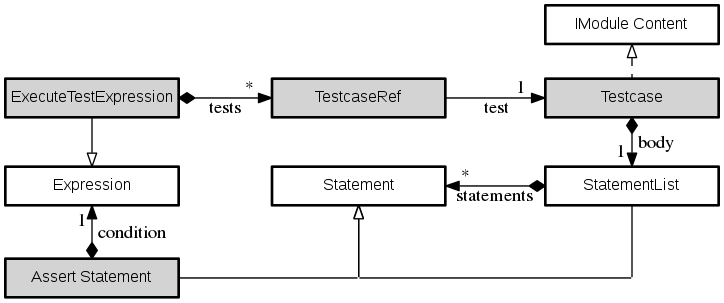
\includegraphics[width=8.5cm]{./figures/unitTestingLangUML2.png} 
    \vspace{-3mm} 
    \caption{Language structure}
  \label{fig:UnitTestStructure}
  \vspace{-5mm}
\end{figure}

\subsection{Type System and Constraints}

\ic{AssertStatemnt} requires a constraint and a type
system rule. First restricts the usages only inside \ic{Testcase}s, meaning an
\ic{AssertStatemnt} can only be used in a \ic{Testcase}:
\begin{lstlisting}[language=constraintsAndTS,frame=single]
parentNode.ancestor<concept = Testcase, +>.isNotNull
\end{lstlisting}

Second restricts the type of its child \ic{expr} (\emph{condition}) to
\ic{BooleanType}, so only valid \emph{conditions} can be entered:
\begin{lstlisting}[language=constraintsAndTS,frame=single]
check(typeof(assertStatement.expr) :<=: <BooleanType()>);
\end{lstlisting}

\ic{ExecuteTestExpression} returns the number of failed unit tests,  
hence we specify \ic{Int32tType} as its type (see rule below). Later the same
type is used in the generator.

\begin{lstlisting}[language=constraintsAndTS,frame=single]
check(typeof(executeTestExpression) :==: <Int32tType()>);
\end{lstlisting}


\subsection{Generator}

The unit testing generator consists of many different transformation rules,
which translate code written with the language directly to mbeddr C. \lst{lst:generatedUT} shows
on the left hand side an example program, written with mbeddr C and the unit
testing language. The right hand side shows the C program generated from it.
While regular mbeddr code is not colored, the boxes show how \ac{AST} nodes from the
left are translated to C code on the right.

\vspace{-2mm}
\noindent 
\hspace{1.2mm}
\begin{minipage}[t]{120pt} 
\begin{lstlisting}[language=reducedMbeddr,numbers=left]
int32 main(int32 argc,
		string[] argv) {
   return $\colorbox{g1}{test[}$$\colorbox{g6}{forTest}$$\colorbox{g1}{]}$;
}
$\colorbox{white}{\hspace{2mm}{\color{white}\_f;}}$
$\colorbox{white}{\hspace{2mm}{\color{white}blockexpr\_2();}}$
$\colorbox{white}{\hspace{2mm}{\color{white}\}}}$
$\colorbox{white}{\hspace{2mm}{\color{white}\}}}$
$\colorbox{white}{\hspace{2mm}{\color{white}int32\_t bp\_2() \{}}$ 
$\colorbox{white}{\hspace{2mm}{\color{white}i32\_t \_f = 0;}}$		

$\colorbox{g7}{testcase forTest \{}$ 
$\colorbox{white}{\hspace{2mm}{\color{white}|}}$
   int32 sum = 0;
$\colorbox{g3}{\hspace{2.5mm}assert:}$ sum == 0$\colorbox{g3}{;}$   
   int32[] nums = {1, 2, 3};
   for(int32_t i=0;i<3;i++){
     sum += nums[i];
   }
$\colorbox{g3}{\hspace{2.5mm}assert:}$ sum == 6$\colorbox{g3}{;}$
$\colorbox{white}{{\color{white}\_f++;}}$
$\colorbox{g7}{\}}$
\end{lstlisting}
\end{minipage} 
\rule[-52ex]{0.1ex}{23.0em}
\hspace{0.75mm}
\begin{minipage}[t]{125pt} 
\begin{lstlisting}[language=reducedMbeddr,numbers=left]
int32_t main(int32_t argc,
		char *(argv[])) {
   return $\colorbox{g1}{blockexpr\_2()}$;
}  
$\colorbox{white}{\hspace{2.5mm}{\color{white}|}}$
$\colorbox{g1}{int32\_t blockexpr\_2(void) \{}$
$\colorbox{g1}{\hspace{2.5mm}int32\_t \_f = 0;}$
$\colorbox{g6}{\hspace{2.5mm}\_f += test\_forTest();}$
$\colorbox{g1}{\hspace{2.5mm}return \_f;}$
$\colorbox{g1}{\}}$

$\colorbox{g7}{int32\_t test\_forTest() \{}$
$\colorbox{g7}{\hspace{2.8mm}int32\_t \_f = 0;}$
   int32_t sum = 0;
$\colorbox{g3}{\hspace{2.8mm}if(!(}$sum == 0$\colorbox{g3}{)) \{ \_f++; \}}$
   int32_t[] nums = {1, 2, 3};
   for(int32_t i=0;i<3;i++){
     sum += nums[i];
   }
$\colorbox{g3}{\hspace{2.8mm}if(!(}$sum == 6$\colorbox{g3}{)) \{ \_f++; \}}$
$\colorbox{g7}{\hspace{2.8mm}return \_f;}$
$\colorbox{g7}{\}}$
\end{lstlisting}
\end{minipage} 
\vspace{-3mm}
\begin{lstlisting}[caption={Example mbeddr program using the unit test language
on the left and the C code that has been generated from it on the right.},
language=mbeddr,label=lst:generatedUT]
\end{lstlisting}

